\documentclass[10pt,svgnames]{beamer}
\usetheme[
%%% option passed to the outer theme
%    progressstyle=fixedCircCnt,   % fixedCircCnt, movingCircCnt (moving is deault)
  ]{Feather}
  
% If you want to change the colors of the various elements in the theme, edit and uncomment the following lines

% Change the bar colors:
%\setbeamercolor{Feather}{fg=red!20,bg=red}

% Change the color of the structural elements:
%\setbeamercolor{structure}{fg=red}

% Change the frame title text color:
%\setbeamercolor{frametitle}{fg=blue}

% Change the normal text color background:
%\setbeamercolor{normal text}{fg=black,bg=gray!10}

%-------------------------------------------------------
% INCLUDE PACKAGES
%-------------------------------------------------------
\usepackage[utf8]{inputenc}
\usepackage[english]{babel}
\usepackage[T1]{fontenc}
\usepackage{helvet}
\usepackage[justification=centering]{caption}
\usepackage{subcaption}
\usepackage{multirow}
%-------------------------------------------------------
% DEFFINING AND REDEFINING COMMANDS

\definecolor{conv}{RGB}{255, 102, 0.0}
\definecolor{pool}{RGB}{255, 223, 51}
\definecolor{drop}{RGB}{173, 220, 83}
\definecolor{citem}{RGB}{15, 88, 11}
\definecolor{elem}{RGB}{0, 112, 255}
%-------------------------------------------------------

% colored hyperlinks
\newcommand{\chref}[2]{
  \href{#1}{{\usebeamercolor[bg]{Feather}#2}}
}

%-------------------------------------------------------
% INFORMATION IN THE TITLE PAGE
%-------------------------------------------------------

\title[ICPRS-18 Conference] % [] is optional - is placed on the bottom of the sidebar on every slide
{ % is placed on the title page
      \textbf{Towards landmarks prediction with Deep Network}
}

%subtitle[The Feather Beamer Theme]
%{
%      \textbf{v. 1.0.0}
%}

\author[V.L. Le, M. Beurton-Aimar, A. Zemmari, N. Parisey]
{      Van-Linh LE$^{1,3}$, Marie BEURTON-AIMAR$^{1}$,\\ Akka ZEMMARI$^{1}$, Nicolas PARISEY$^{2}$ \\[0.4cm]
      {\ttfamily\footnotesize{linhlv@dlu.edu.vn/van-linh.le@labri.fr, beurton@labri.fr\\
		akka.zemmari@labri.fr, nicolas.parisey@inra.fr \\    }
      }
}

\institute[]
{
      $^1$LaBRI-CNRS 5800, Bordeaux University, France\\
      $^2$IGEPP, INRA 1349 Rennes, France\\
      $^3$ITDLU, Dalat University, Vietnam
  
  %there must be an empty line above this line - otherwise some unwanted space is added between the university and the country (I do not know why;( )
}
\date[ICPRS-2018]{\textbf{ICPRS Conference}\\Valparaíso, 22-24 May, 2018}
%\date{\today}

%-------------------------------------------------------
% THE BODY OF THE PRESENTATION
%-------------------------------------------------------

\begin{document}

%-------------------------------------------------------
% THE TITLEPAGE
%-------------------------------------------------------

{\1% % this is the name of the PDF file for the background
\begin{frame}[plain,noframenumbering] % the plain option removes the header from the title page, noframenumbering removes the numbering of this frame only
  \titlepage % call the title page information from above
\end{frame}}

%-------------------------------------------------------

\begin{frame}[t]{Context}
%-------------------------------------------------------
\begin{block}{Morphometry analysis}
  \begin{itemize}    
    \item Used to study the complex interaction between the morphometry of species and environmental factors.
    \item Characterize information of biological species such as shape, sizes, or \textbf{landmarks},\ldots.
  \end{itemize}
  \end{block}

  \begin{block}{Landmark}
  \begin{itemize}
     \item A kind of \textbf{point of interest} 
     \item A specific point defined by biologist. For example, intersection of veins on fly wing, the corner of beetle's pronotum shape,\ldots
  \end{itemize}
  	\begin{figure}[htbp]
       \centering
       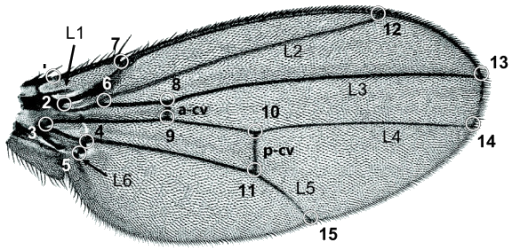
\includegraphics[scale=.17]{images/wing}~~~~~~
       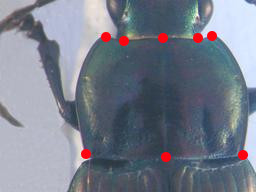
\includegraphics[scale=.3]{images/pronotum_lm}~~
	\end{figure}
  \end{block}
\end{frame}

%-------------------------------------------------------

%-------------------------------------------------------

\begin{frame}[c]{Dataset}
%-------------------------------------------------------
	\begin{itemize}
    	\item Images have been taken from $293$ \textbf{beetles}, seperate into 5 parts,
    	\item Format: $2$D in RGB color,
    	\item Focus on \textbf{\color{red}pronotum} images.
  	\end{itemize}
	
	\begin{figure}[htbp]
    			\begin{subfigure}[t]{0.3\textwidth}
        			\centering
        			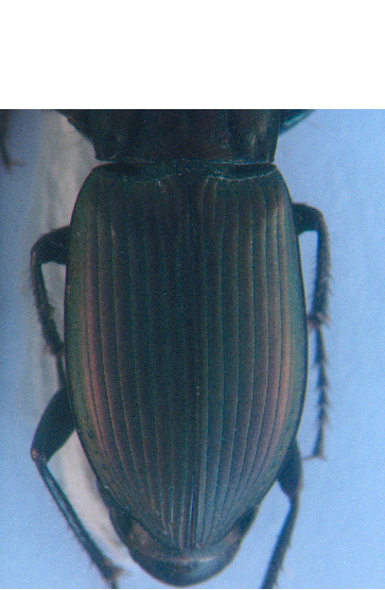
\includegraphics[scale=.2]{images/elytre2}
        			\caption*{\footnotesize{Body part/elytre}}
        			\label{figsub22}
    			\end{subfigure}
    			~ 
    			\begin{subfigure}[t]{0.3\textwidth}
        			\centering
        			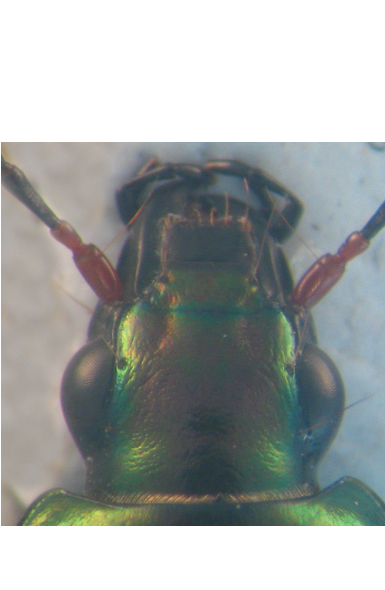
\includegraphics[scale=.2]{images/tete2}
        			\caption*{\footnotesize{Head part/tete}}
        			\label{figsub22}
    			\end{subfigure}
    			~ 
    			\begin{subfigure}[t]{0.33\textwidth}
        			\centering
        			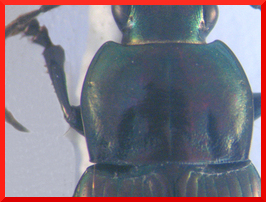
\includegraphics[scale=1.1]{images/pronotum}
        			\caption*{\footnotesize{Pronotum part}}
        			\label{figsub22}
    			\end{subfigure}
			\end{figure}
\end{frame}

%-------------------------------------------------------

\begin{frame}{Landmark setting}{}
%-------------------------------------------------------
	\begin{block}{Manual landmarks}		
		\begin{itemize}
	  				\item Time-consuming
					\item Difficult to reproduce
  				\end{itemize}
	\end{block}
	\begin{block}{Problems}
		\begin{columns}
			\begin{column}{0.65\textwidth}
				Pronotum image:
				\begin{itemize}
  					\item Not precised: contains also a part of head and body
		  			\item Difficult to segment this object
  					\item The landmarks are set both on the shape and inside the object
  				\end{itemize}
			\end{column}
			\begin{column}{0.3\textwidth}
				\begin{figure}[htbp]
					\centering
					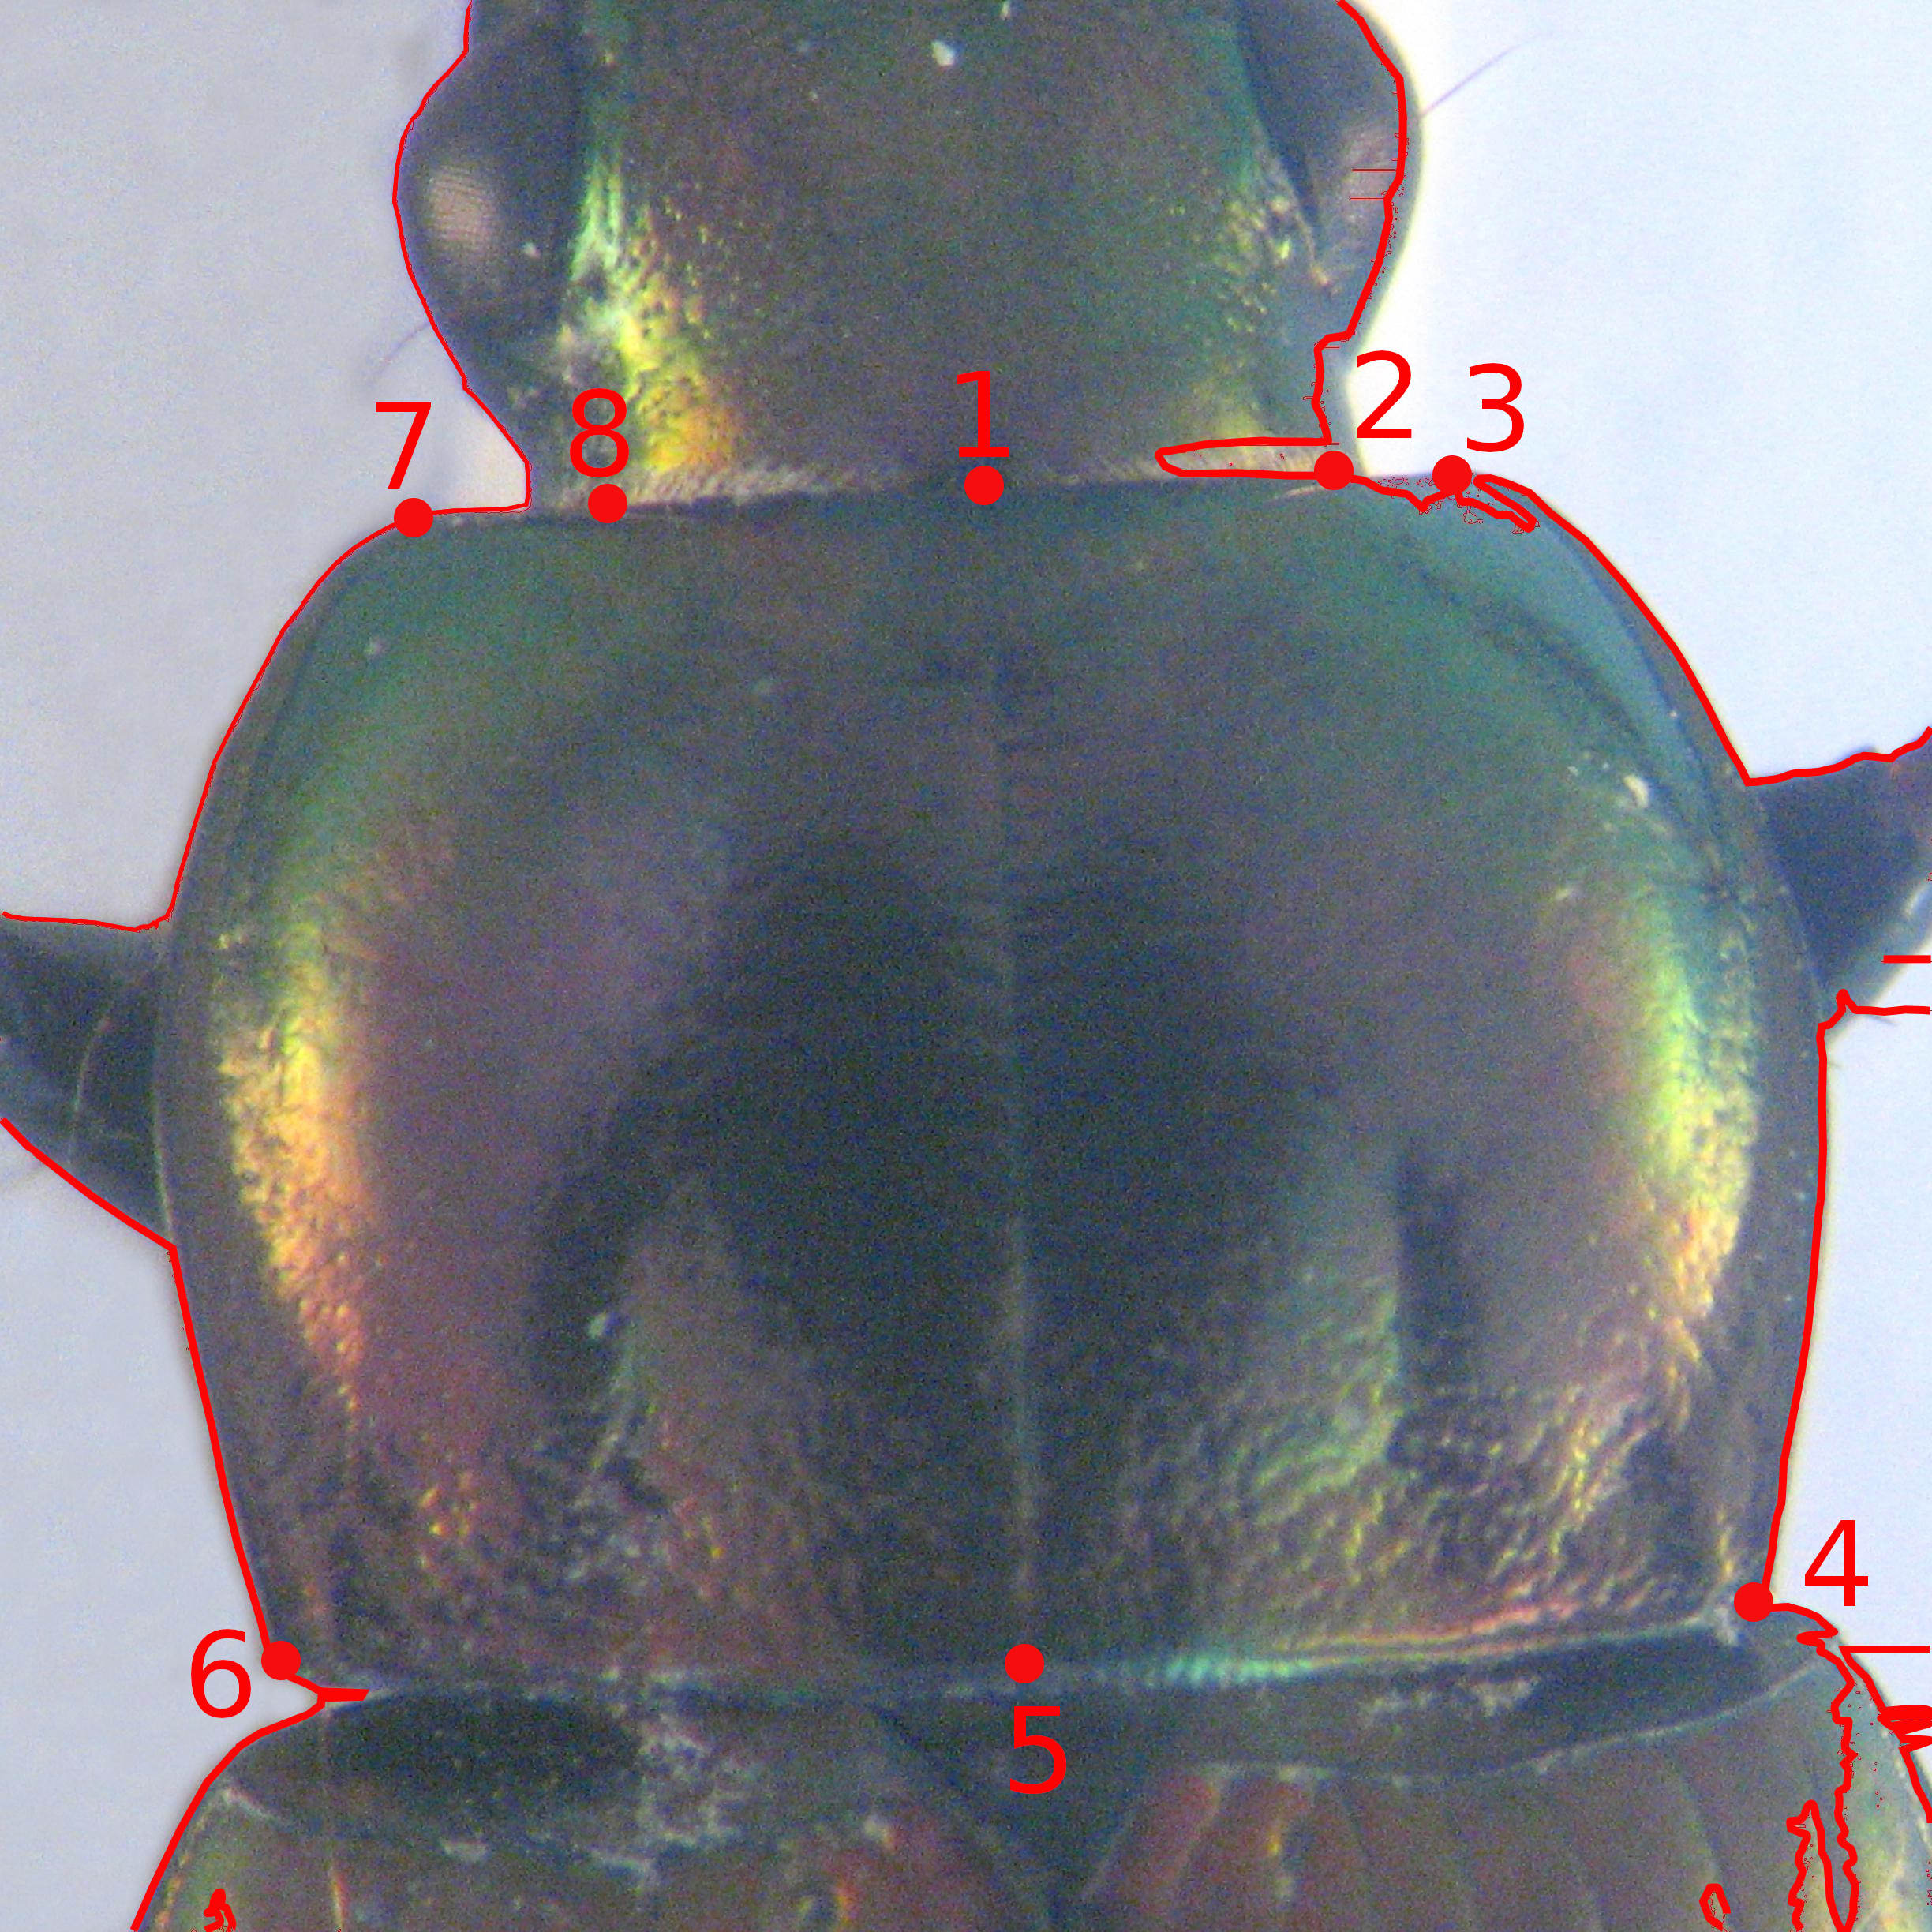
\includegraphics[scale=.040]{images/prono_003_lm2}
				\end{figure}
			\end{column}
		\end{columns}		
	\end{block}
	\pause
	\begin{center}	
		\textbf{How to {\color{red}automatically} predict the {\color{red}landmarks coordinates}?}	
	\end{center}
  	
  
	
\end{frame}

%-------------------------------------------------------
\begin{frame}{Content}{}
\tableofcontents
\end{frame}
%-------------------------------------------------------
\section{Deep learning and Convolutional Neural Networks}
\subsection{Deep learning}
%-------------------------------------------------------
\begin{frame}{Deep learning}{}
	\only<1-2>{
	\begin{block}{Definition\footnotemark[1]}
		\begin{itemize}
			\item A class of machine learning methods.
			\item Use a cascade of multiple layers for feature extraction and transformation.
			\item Learn multiple levels of representation in supervised or unsupervised mode.
		\end{itemize}
	\end{block}{\footnotetext[1]{\tiny{Y. LeCun, Y. Bengio, and G. Hinton, “Deep learning,” Nature, vol. 521, no. 7553, pp. 436–444, 2015}}}
	}
	\only<2>{
	\begin{block}{Applications}
		\begin{itemize}
			\item Computer vision (image recognition and classification)
			\item Speech recognition
			\item Question answering, language translation, \ldots
		\end{itemize}
	\end{block}
	}
\end{frame}
%-------------------------------------------------------
\subsection{Convolutional neural networks (CNNs)}
%-------------------------------------------------------
\begin{frame}{Convolutional neural networks}
	\begin{itemize}
		\item Consists an input, an output and multiple hidden layers\footnotemark[1]
		\item Arranges the data in $3$ dimensions: \textit{width, height and depth}
		\item Classical layers: \textbf{\color{conv}convolutional} layers, \textbf{\color{pool}pooling} layers, \textbf{\color{drop}dropout} layers, \textbf{\color{blue}full-connected} layers, \ldots
	\end{itemize}
	\begin{figure}[htbp]
  		\centering
   	 	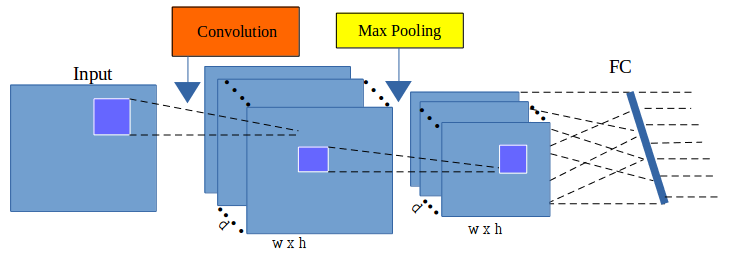
\includegraphics[scale=.27]{images/arch_cnn1}
   	 	%\caption{\footnotesize{An example of CNN}}
	\end{figure}
	\footnotetext[1]{
		\tiny{
			Y. LeCun et al, ``Convolutional networks
and applications in vision", 2010.
		}
	}
\end{frame}
%-------------------------------------------------------
\section{Proposed method}
\subsection{Network architectures}
%-------------------------------------------------------
%-------------------------------------------------------
\begin{frame}{First architecture}{}
	The first applied networks:
	\begin{itemize}
		\item Repeat the pair of {\color{conv}convolutional} and {\color{pool}maximum pooling} layers
		\item Trying to adjust the parameters of the layers
	\end{itemize}
	\begin{center}
   		\begin{figure}[htbp]
   			\centering
    		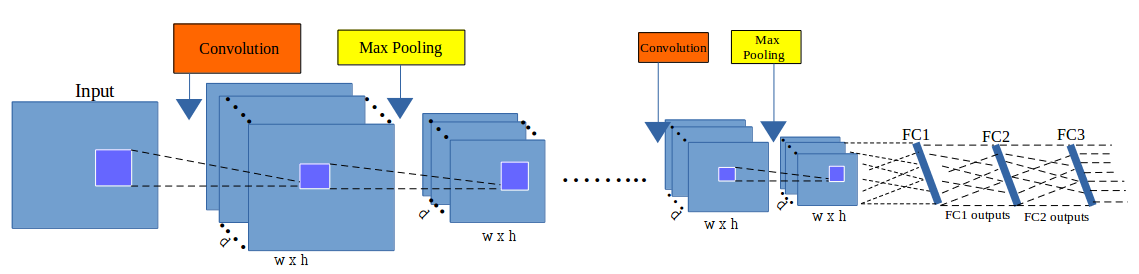
\includegraphics[scale=.28]{images/arch_cnn2}    
		\end{figure}
   \end{center}
\end{frame}
%-------------------------------------------------------
\begin{frame}{Our proposed architecture}{Elementary block}
  \begin{columns}
		\begin{column}{0.45\textwidth}	
			
			\textbf{\color{elem}Elementary block}: 
			\small{
			\begin{itemize}
				\item A \textbf{\color{conv}convolutional} layer
    			\item A \textbf{\color{pool}maxixum pooling} layer
    			\item A \textbf{\color{drop}dropout} layer
  			\end{itemize}  			
  			}			 			
		\end{column}
		\begin{column}{0.55\textwidth}  %%<--- here
			\begin{center}
     			\begin{figure}[htbp]
        			\centering
        			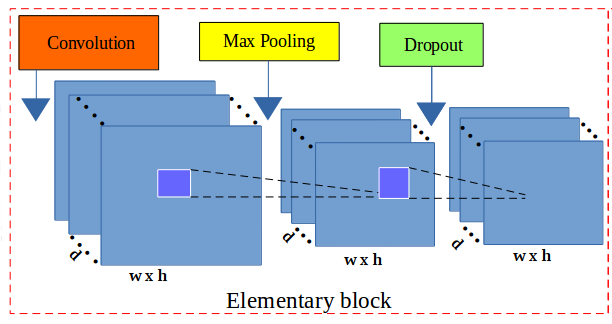
\includegraphics[scale=.28]{images/elementary_block}
        			%\caption{\footnotesize{Pronotum}}
    				\label{figrsexample1}
				\end{figure}
     		\end{center}	     					     		
		\end{column}
	\end{columns}~\\		
		
\end{frame}

%-------------------------------------------------------
\begin{frame}{Our proposed architecture}{Elementary blocks composition}
	The proposed model: 
		\small{
			\begin{itemize}
				\item \textbf{Three} \textbf{\color{elem}elementary blocks}
    			\item \textbf{Three} {\color{blue}full-connected} (FC) layers
    			\item A dropout layer was inserted between the first and the second FC layer
  			\end{itemize}}
  		
    		\begin{center}
     			\begin{figure}[htbp]
        			\centering
        			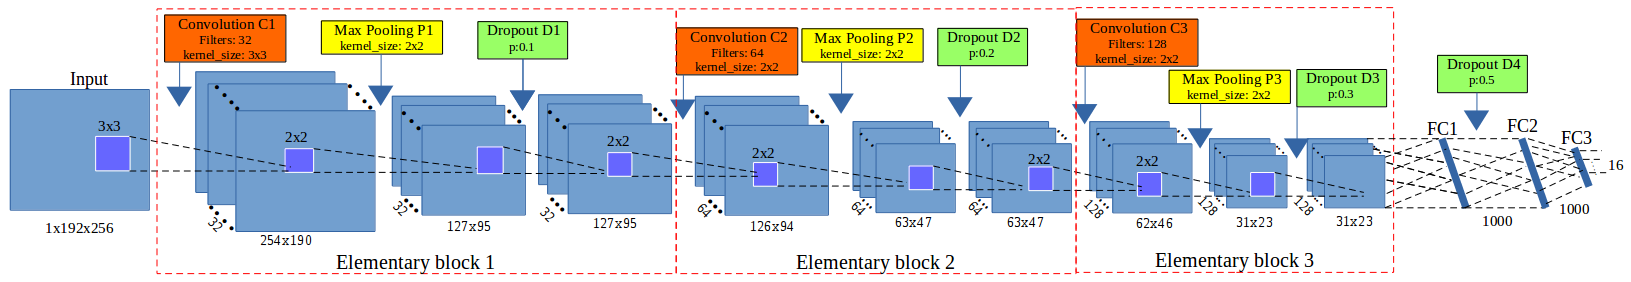
\includegraphics[scale=.2]{images/arch_model}
				\end{figure}
     		\end{center}
\end{frame}
%-------------------------------------------------------
\subsection{Data augmentation}
%-------------------------------------------------------
\begin{frame}{Data augmentation}{}
	\only<1-3>{Dataset: {\color{red}$293$ pronotum}  images in {\color{red}R}{\color{green}G}{\color{blue}B} format.\\}
	\only<1-3>{Augmentation methods:
	\begin{itemize}
		\only<1,3>{\item Increase the value of each channel}
		\only<2,3>{\item Split the channels}
	\end{itemize}
	}
	\only<3>{$\Rightarrow$ Total: $293 \times 7 = 2,051$ images}
\only<1>{
  \begin{center}
     \begin{figure}[htbp]
        \centering
        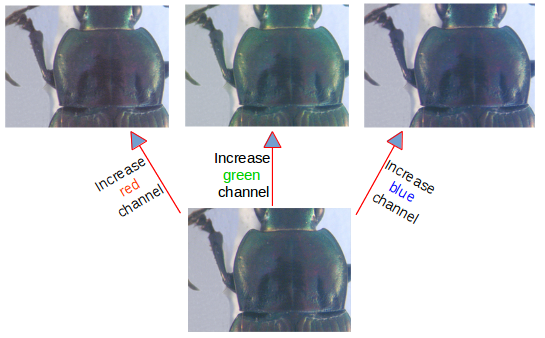
\includegraphics[scale=.45]{images/inc_channels}
       	%\caption{\footnotesize{Pronotum}}
    	\label{figrsexample1}
	\end{figure}
  \end{center}
  }
 \only<2>{
  \begin{center}
     \begin{figure}[htbp]
        \centering
        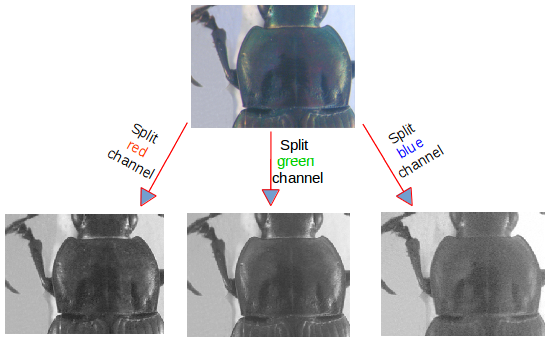
\includegraphics[scale=.45]{images/sp_channels}
       	%\caption{\footnotesize{Pronotum}}
    	\label{figrsexample1}
	\end{figure}
  \end{center}
  }
  \only<3>{
  \begin{center}
     \begin{figure}[htbp]
        \centering
        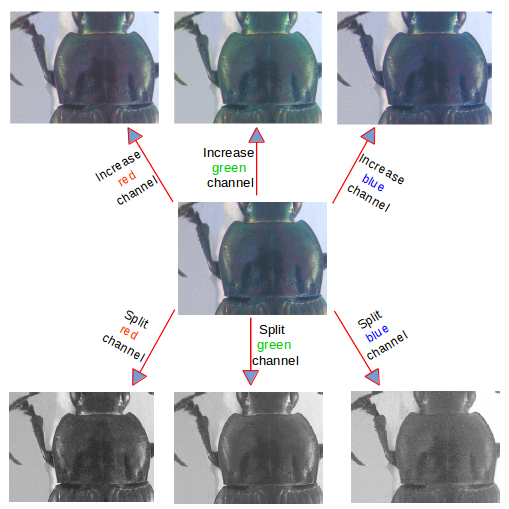
\includegraphics[scale=.25]{images/data_aug}
       	%\caption{\footnotesize{Pronotum}}
    	\label{figrsexample1}
	\end{figure}
  \end{center}
  }

\end{frame}
%-------------------------------------------------------
\section{Results}
\subsection{Training from scratch}
%-------------------------------------------------------
\begin{frame}{Training}{}
	\begin{itemize}
		\item Training dataset: \textbf{$1,820$} images ($260 \times 7$)
		\item Apply the cross-validation to select training and testing data
		\item Training parameters: momentum ($0.9 \rightarrow 0.9999$), learning rate ($0.03 \rightarrow 0.00001$), $5000$ epochs\footnotemark
		\item Image shows training and validation losses of the model
		\item Training time: 3 hours using NVIDIA TITAN X card
	\end{itemize}
	\begin{center}
     \begin{figure}[htbp]
        \centering
        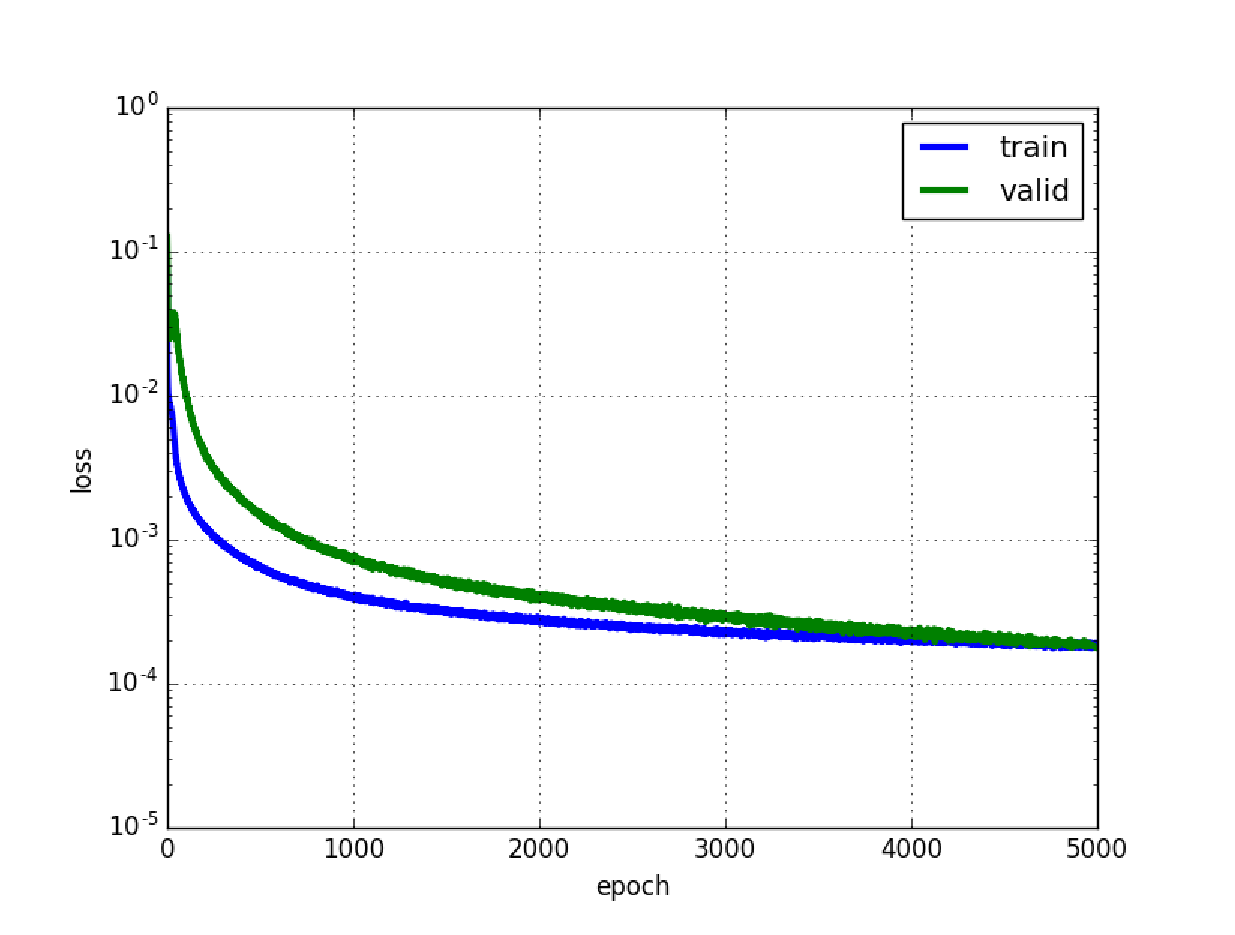
\includegraphics[scale=.30]{images/loss_model_3}
       	%\caption{\footnotesize{Pronotum}}
    	\label{figrsexample1}
	\end{figure}
  \end{center}
	
	\footnotetext{\tiny{An epoch is a single pass through the full training set.}}
\end{frame}

\begin{frame}{First results}{Correlation metrics and landmarks on the images}
	\begin{itemize}
		\item Quality metrics: coefficient of determination ($r^2$), explained variance (EV), Pearson correlation.
			\begin{table}[htbp]
				\centering
				\begin{tabular}{|c|p{1cm}|p{1cm}|p{1.5cm}|}
					\hline
					Metric & $\mathbf{r^{2}}$ & \textbf{EV} & \textbf{Pearson} \\ \hline
					Proposed architecture & $\textbf{0.9952}$ & $\textbf{0.9951}$ & $\textbf{0.9974}$ \\ \hline
				\end{tabular}
			\end{table}~\\
	\pause
	\item Display the landmarks on the images:
	\begin{figure}[htbp]
   				\begin{subfigure}[t]{0.5\textwidth}
        			\centering
        			\includegraphics[scale=.135]{images/plandmark}
        			\caption{ }
        			\label{figsub11}
    			\end{subfigure}%
    			~ 
    			\begin{subfigure}[t]{0.5\textwidth}
        			\centering
        			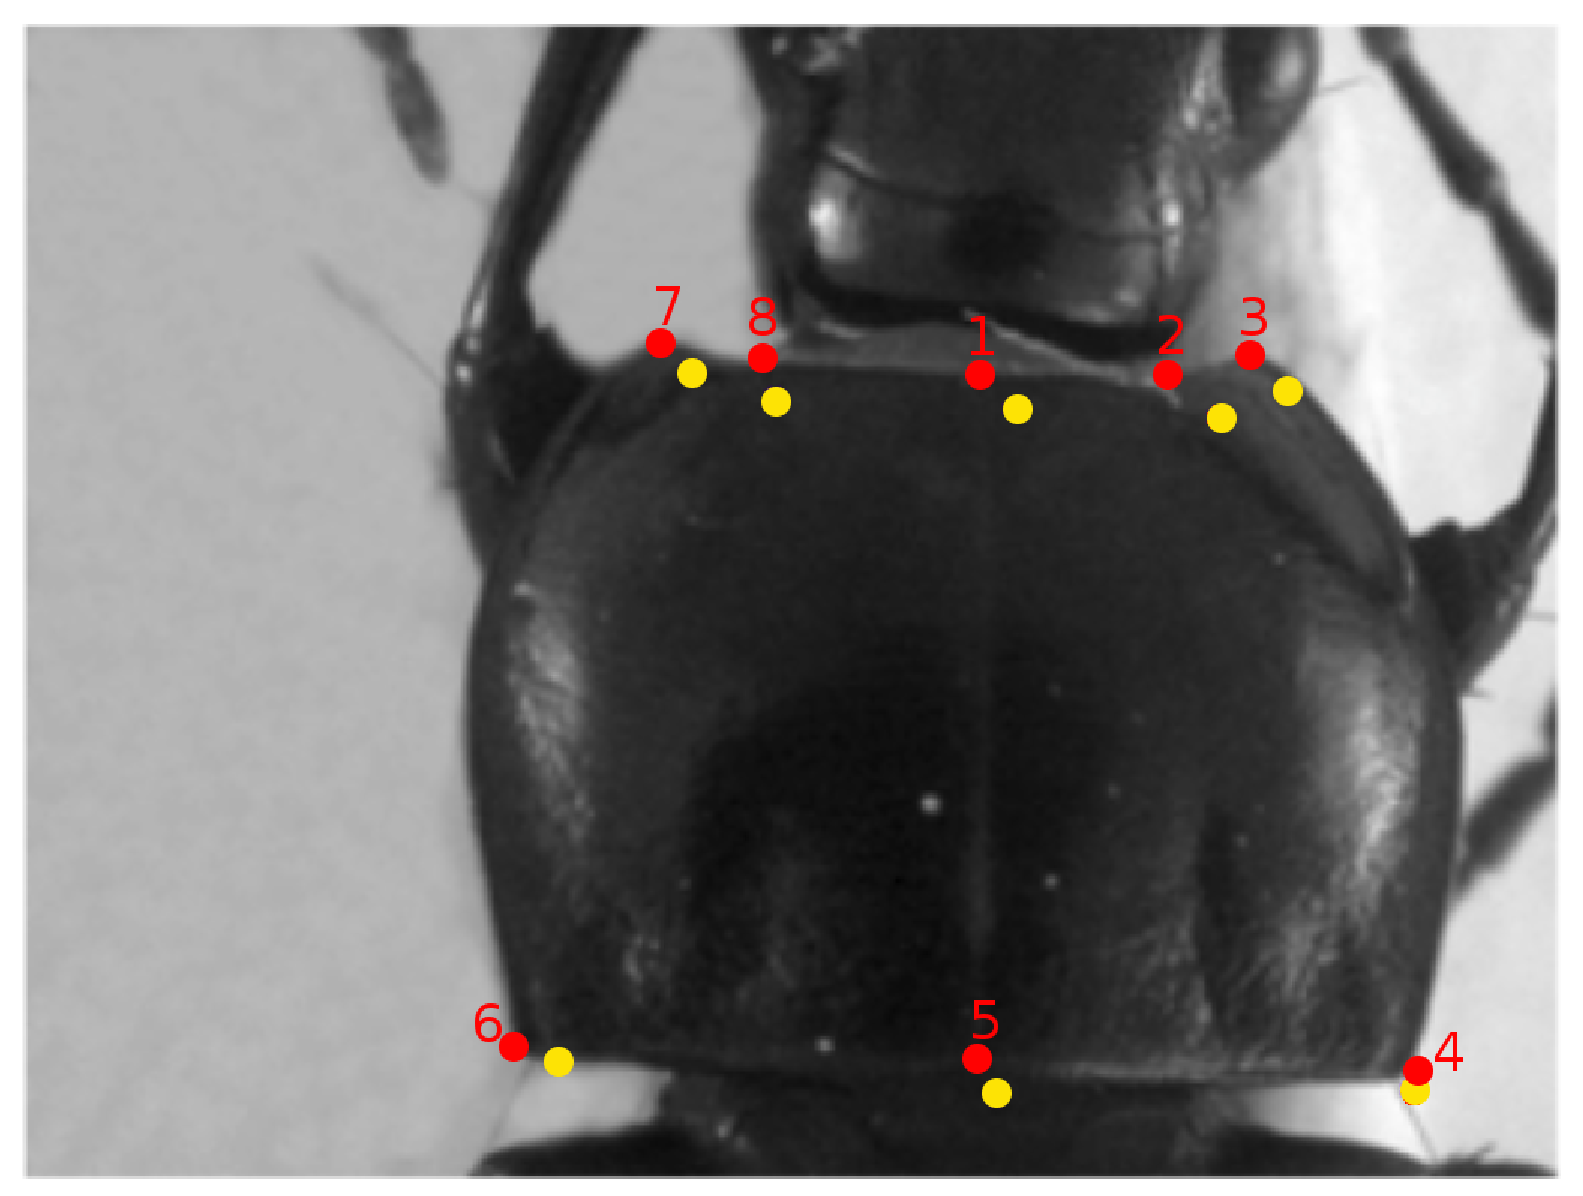
\includegraphics[scale=.2]{images/plandmark2}
        			\caption{ }
        			\label{figsub22}
    			\end{subfigure} 
    		\end{figure}
   	\end{itemize}
\end{frame}


%-------------------------------------------------------

\begin{frame}{First results}{Average distances}
	\begin{itemize}			
		\item Calculate the distance between predicted landmarks and corresponding manual landmarks.	
		\item Compute the average distance by landmark.\\
		
			\begin{table}[htbp]
				\centering
				\begin{tabular}{|c|c|}
					\hline
					\textbf{Landmark} & \textbf{Distance} (in pixels) \\ \hline
					\textbf{\color{green}1} & \textbf{\color{green}4.002}  \\ \hline
					2 & 4.4831 \\ \hline
					3 & 4.2959 \\ \hline
					4 & 4.3865 \\ \hline
					5 & 4.2925 \\ \hline
					\textbf{\color{red}6} & \textbf{\color{red}5.3631} \\ \hline
					7 & 4.636 \\ \hline
					8 & 4.9363 \\ \hline
				\end{tabular}
				\caption*{The statistic of average distances on all images per landmark.}
			\end{table}
	\end{itemize}
\end{frame}

%-------------------------------------------------------
\subsection{Fine-tuning}
\begin{frame}{Transfer learning/Knowledge transfer}{}
	\begin{itemize}
		\item Re-use model developed for a specific task/dataset to lead another task on another dataset
		\item \textbf{Fine-tuning}: retrain a pretrained model
		\item \textbf{Model Zoo} (Caffe library): people share their pre-trained networks.
	\end{itemize}				
	\begin{center}
     \begin{figure}[htbp]
        
\includegraphics[scale=.2]{images/transfer_learning_2x}\\[-1ex]     	
	\end{figure}
  \end{center}
  {\tiny Image source: \textbf{DataCamp}}
\end{frame}
%-------------------------------------------------------
\begin{frame}{Fine-tuning our model}{}
	\only<1-2>{	
	\begin{itemize}
		\item Estimated landmarks on pronotum images when fine-tuning on \textbf{VGG-16, VGG-19, ResNet50} have not been improved
		\item Train the model on a dataset including the images of $3$ parts of beetles: head, body and pronotum parts \textbf{($5,460$ images)}
		\item Fine-tune pretrained model on pronotum dataset
	\end{itemize}
	}
	\only<1>{				
	\begin{center}
     \begin{figure}[htbp]
        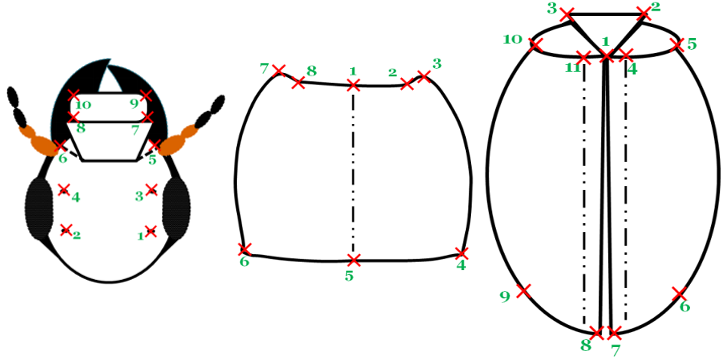
\includegraphics[scale=.4]{images/merge}   	
	 \end{figure}
    \end{center}
    }
    \only<2>{
    \begin{center}
     \begin{figure}[htbp]
        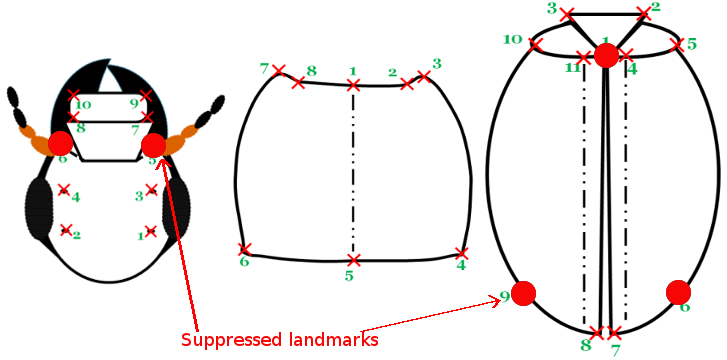
\includegraphics[scale=.4]{images/merge_rm}
    	\label{figrsexample1}
	 \end{figure}
    \end{center}
    }
\end{frame}
%-------------------------------------------------------

\begin{frame}{Results}{A comparation of average distances}
	
	Comparing the average distances between two processes: training from scratch and fine-tuning.
	\begin{table}[htbp]
		\centering
		\begin{tabular}{ | c | c | c | c | c | }
			\hline
	
			\multicolumn{1}{|c|}{\multirow{2}{*}{Landmarks}} & \multicolumn{2}{c|}{From scratch} &  \multicolumn{2}{c|}{With fine-tuning}  \\ \cline{2-5}
	 & Average & SD & Average & SD \  \\ \hline
			\color{green}{\textbf{LM1}} & \color{green}{\textbf{4.002}} & \color{green}{\textbf{2.5732}} & \color{green}{\textbf{2.486}} & \color{green}{\textbf{1.5448}} \\ \hline
			LM2 & 4.4831 & 2.7583 & 2.7198 & 1.7822 \\ \hline
			LM3 & 4.2959 & 2.7067 & 2.6523 & 1.8386 \\ \hline
			LM4 & 4.3865 & 3.0563 & 2.7709 & 1.9483 \\ \hline
			LM5 & 4.2925 & 2.9086 & 2.4872 & 1.6235 \\ \hline
			\color{red}{\textbf{LM6}} & \color{red}{\textbf{5.3631}} & \color{red}{\textbf{3.4234}} & \color{red}{\textbf{3.0492}} & \color{red}{\textbf{1.991}} \\ \hline
			LM7 & 4.636 & 2.8426 & 2.6836 & 1.7781 \\ \hline
			LM8 & 4.9363 & 3.0801 & 2.8709 & 1.9662 \\ \hline
		\end{tabular}
	\end{table}
	
\end{frame}
\begin{frame}{Results}{Distribution of average distances}
	
	\begin{itemize}
		\only<1>{
		\item The distribution of distance of the best result ($1^{st}$ landmark)
		\begin{figure}[htbp]
   				\begin{subfigure}[t]{0.5\textwidth}
        			\centering
        			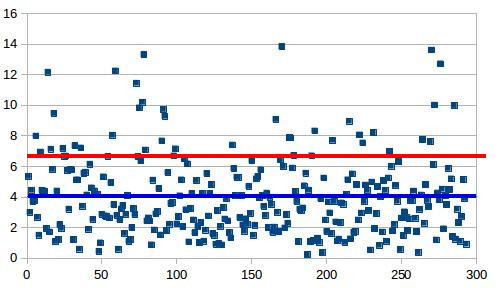
\includegraphics[scale=.4]{images/lm1_cnn_2}
        			\caption{Training from scratch}
    			\end{subfigure}%
    			~ 
    			\begin{subfigure}[t]{0.5\textwidth}
        			\centering
        			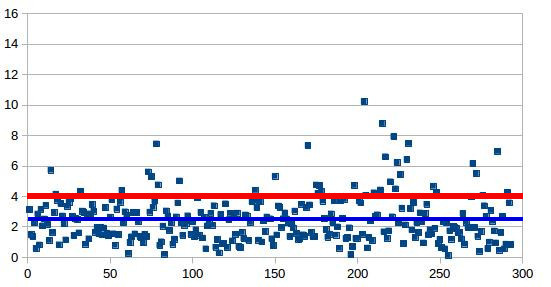
\includegraphics[scale=.38]{images/lm1_finetuning_2}
        			\caption{With fine-tuning}
    			\end{subfigure}    		
			\end{figure}
			}
		\only<2>{
		\item The distribution of distance of the worst result ($6^{th}$ landmark)
		\begin{figure}[htbp]
   				\begin{subfigure}[t]{0.5\textwidth}
        			\centering
        			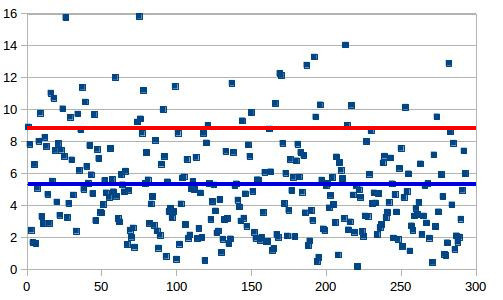
\includegraphics[scale=.4]{images/lm6_cnn_2}
        			\caption{Training from scratch}
    			\end{subfigure}%
    			~ 
    			\begin{subfigure}[t]{0.5\textwidth}
        			\centering
        			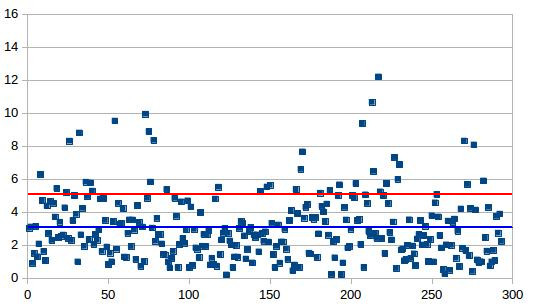
\includegraphics[scale=.38]{images/lm6_finetuning_2}
        			\caption{With fine-tuning}
    			\end{subfigure}    		
			\end{figure}
		}
	\end{itemize}

\end{frame}
%-------------------------------------------------------
\section{Conclusion}
\begin{frame}{Conclusion}
%-------------------------------------------------------
	\begin{block}{Conclusion}
		\small{
			\begin{itemize}
				\item Propose a new CNN architecture with elementary blocks to predict the landmarks on pronotum images.
				\item Propose a new procedure to augment the dataset.
				\item Apply fine-tuning to improve the quality of predicted landmarks.
				\item[\textcolor{citem}{$\bullet$}] The predicted landmarks able to replace the manual landmarks without segmentation step.
			\end{itemize}
		}
	\end{block}
	\pause
	\begin{block}{Future works}
		\small{
			\begin{itemize}
				\item Applying the method on body and head parts 
				\item Going deeply how to design the right pre-training model
			\end{itemize}					
			}
	\end{block}
\end{frame}
%-------------------------------------------------------

{\1
\begin{frame}[plain,noframenumbering]
  \finalpage{\textbf{\color{red}Thank you for attention!}}
\end{frame}}

\end{document}






\begin{frame}{Result}{Statistic on acceptable predicted landmarks}
Chart shows the propotion of acceptable predicted landmarks
\footnotesize{
	\begin{itemize}
		\item Average accuracy: $\sim 75\%$
		\item Highest accuracy: $87.88\%$
		\item Lowest accuracy: $66.67\%$
	\end{itemize}
	}
	\begin{figure}[htbp]
		\centering
		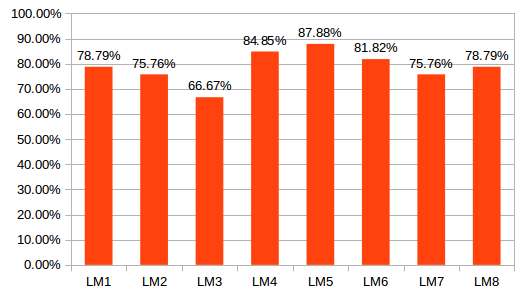
\includegraphics[scale=.6]{images/chart2}	
	\end{figure}
\end{frame}
%-------------------------------------------------------
\begin{frame}{Result}{Distribution of distance on the first landmark}
\small{
	\begin{itemize}
		\item Good prediction: $56.66\%$
		\item Acceptable prediction: $40.27\%$
		\item Bad prediction: $3.07\%$
	\end{itemize}
	}
	\begin{figure}[htbp]
		\centering
		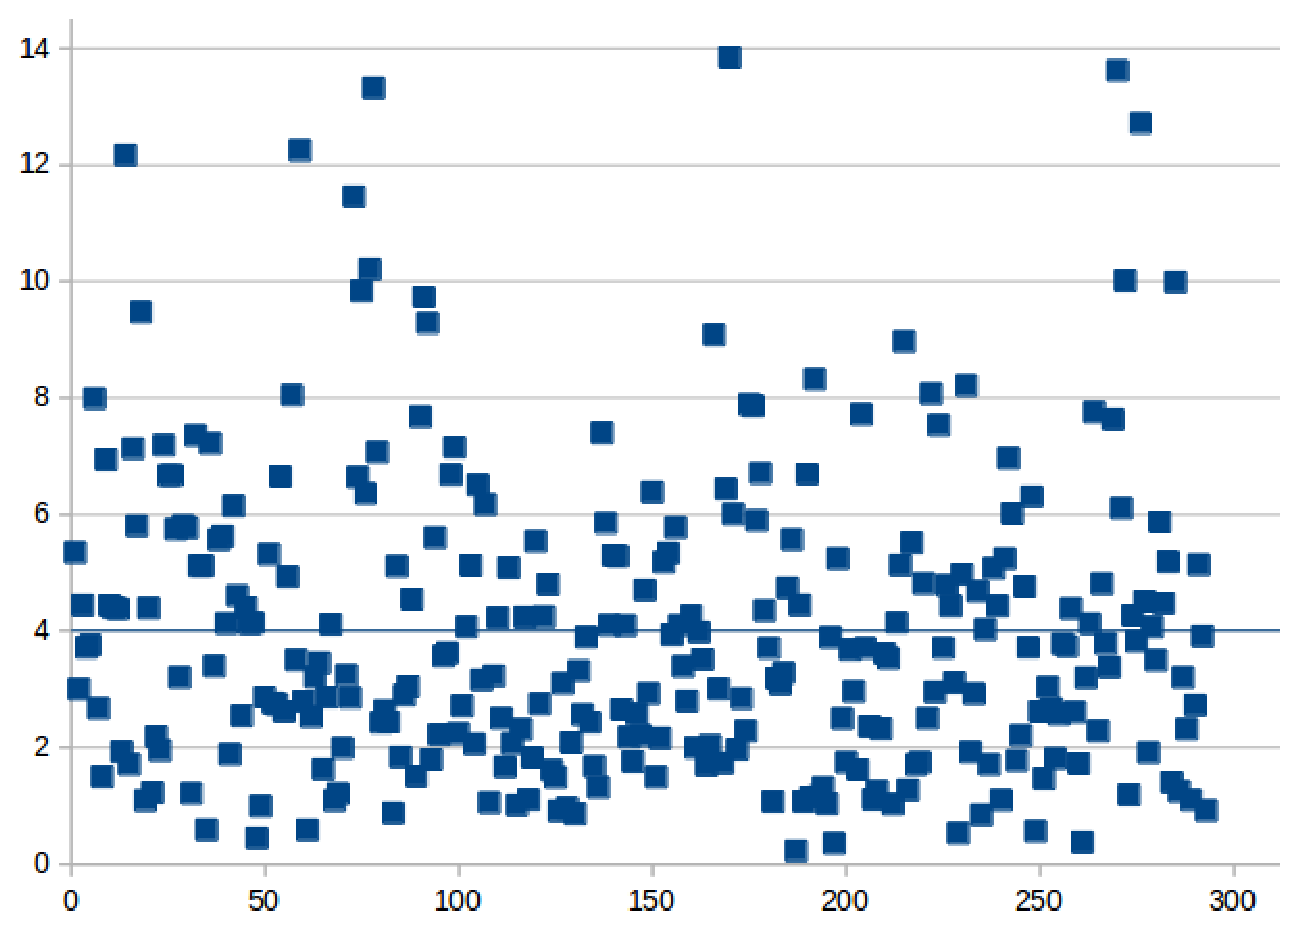
\includegraphics[scale=.3]{images/statistic}	
	\end{figure}
\end{frame}
%-------------------------------------------------------
\begin{frame}{Result}{Comparing with related works}
\small{Quality metrics: coefficient of determination ($r^2$), explained variance (EV), Pearson correlation.
	}
	\begin{table}[htbp]
\centering
\begin{center}
\begin{tabular}{|c|p{1cm}|p{1cm}|p{1.5cm}|}
\hline
Metric & $\mathbf{r^{2}}$ & \textbf{EV} & \textbf{Pearson} \\ \hline
Cintast et al.\footnotemark & $0.884$ & $0.951$ & $0.976$ \\ \hline
Proposed architecture & $\textbf{0.9952}$ & $\textbf{0.9951}$ & $\textbf{0.9974}$ \\ \hline
\end{tabular}
\label{tab3}
\end{center}
\end{table}
\footnotetext{\tiny{Cintas, ``Automatic ear detection and feature extraction using
geometric morphometrics and convolutional neural networks," IET Biometrics, vol. 6, no. 3, pp. 211–223, 2016}}
\end{frame}

\begin{subfigure}[t]{0.22\textwidth}
        			\centering
        			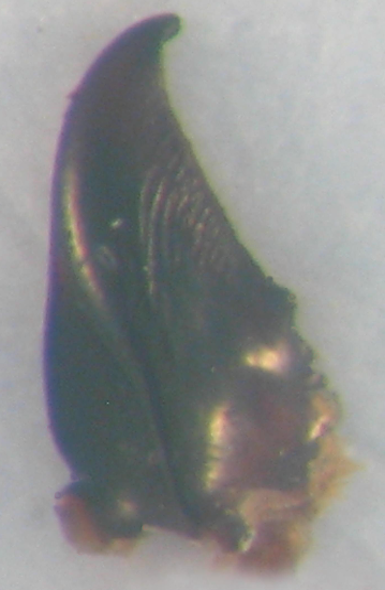
\includegraphics[scale=.13]{images/mgmo}
        			\caption{\footnotesize{Left mandible}}
        			\label{figsub11}
    			\end{subfigure}%
    			~ 
    			\begin{subfigure}[t]{0.22\textwidth}
        			\centering
        			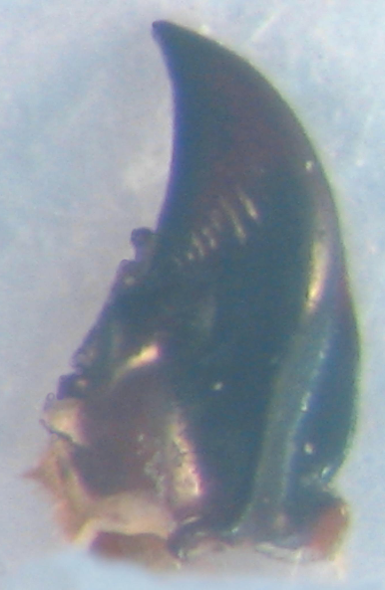
\includegraphics[scale=.13]{images/mdmo}
        			\caption{\footnotesize{Right mandible}}
        			\label{figsub22}
    			\end{subfigure}

\begin{frame}{First result}{Landmarks on images}
%-------------------------------------------------------
\begin{itemize}
		\item Run the trained model to predict the landmarks on testing images,
		\item Calculate the distance between predicted landmarks and corresponding manual landmarks,		
	\end{itemize}
			\begin{figure}[htbp]
   				\begin{subfigure}[t]{0.5\textwidth}
        			\centering
        			\includegraphics[scale=.135]{images/plandmark}
        			\caption{ }
        			\label{figsub11}
    			\end{subfigure}%
    			~ 
    			\begin{subfigure}[t]{0.5\textwidth}
        			\centering
        			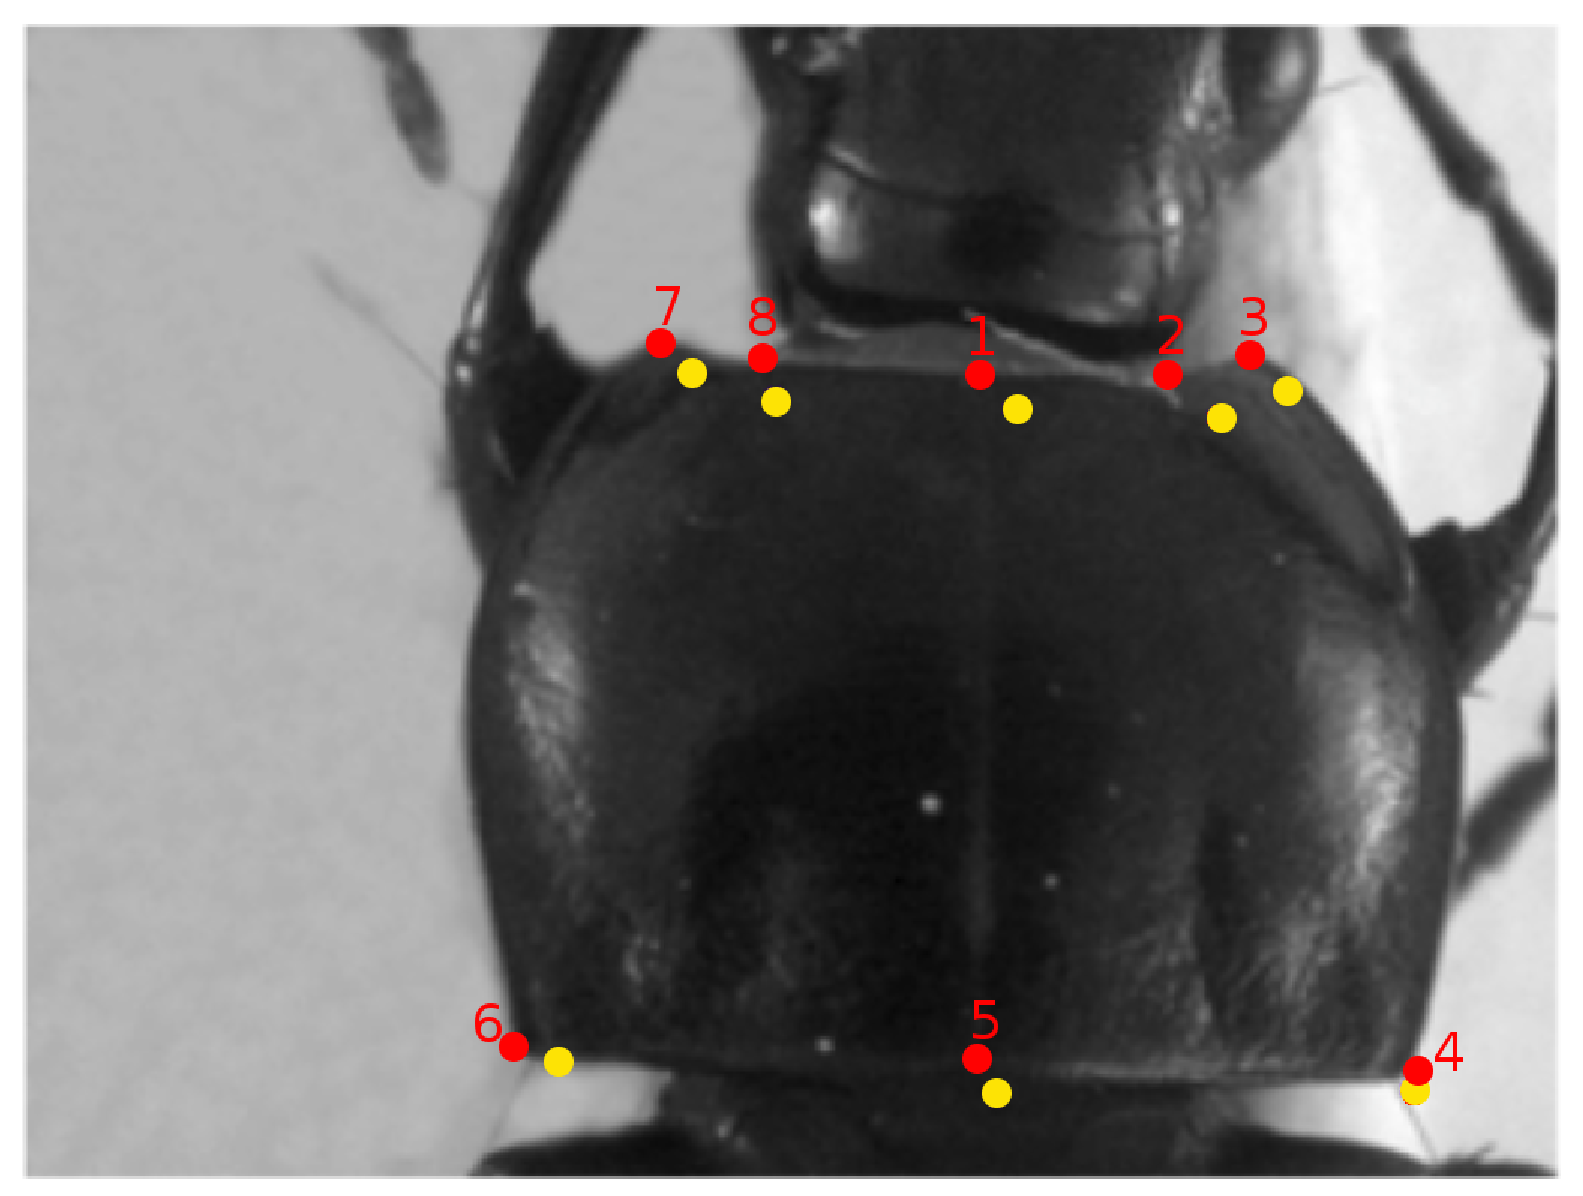
\includegraphics[scale=.2]{images/plandmark2}
        			\caption{ }
        			\label{figsub22}
    			\end{subfigure}    		    			
			\end{figure}
\end{frame}    			


\begin{frame}[c]{Dataset}
%-------------------------------------------------------
	\begin{columns}
		\begin{column}{0.5\textwidth}
			\begin{itemize}
    			\item Images have been taken from $293$ \textbf{beetles}, seperate into 5 parts (images),
    			\item Format: $2$D in RGB color,
    			\item Focus on \textbf{\color{red}pronotum} images.
  			\end{itemize}
		\end{column}
		\begin{column}{0.5\textwidth}  %%<--- here
    		\begin{center}
     			\begin{figure}[htbp]
        			\centering
        			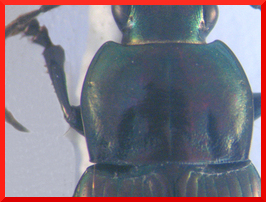
\includegraphics[scale=0.8]{images/pronotum}
        			\caption*{\footnotesize{Pronotum part}}
    				\label{figrsexample1}
				\end{figure}
     		\end{center}
		\end{column}
	\end{columns}
	\begin{figure}[h]
    			\begin{subfigure}[t]{0.3\textwidth}
        			\centering
        			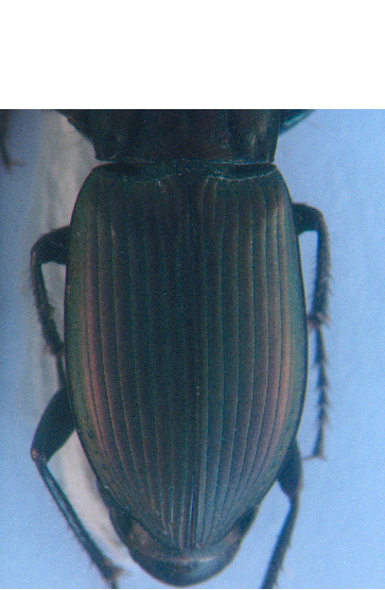
\includegraphics[scale=.15]{images/elytre2}
        			\caption*{\footnotesize{Body part}}
        			\label{figsub22}
    			\end{subfigure}
    			~ 
    			\begin{subfigure}[t]{0.3\textwidth}
        			\centering
        			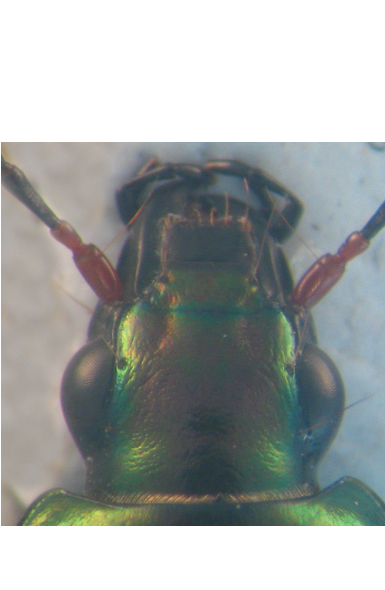
\includegraphics[scale=.15]{images/tete2}
        			\caption*{\footnotesize{Head part}}
        			\label{figsub22}
    			\end{subfigure}
    			
\end{frame}
\begin{frame}{Problems}{}
%-------------------------------------------------------
	Pronotum image:
  	\begin{itemize}
  		\item Very noise: it connects to a part of head and body
  		\item Difficult to segment the object
  		\item The landmarks stay both on the shape and inside the object
  	\end{itemize}
  \begin{figure}[htbp]
        \centering
        \only<1>{
        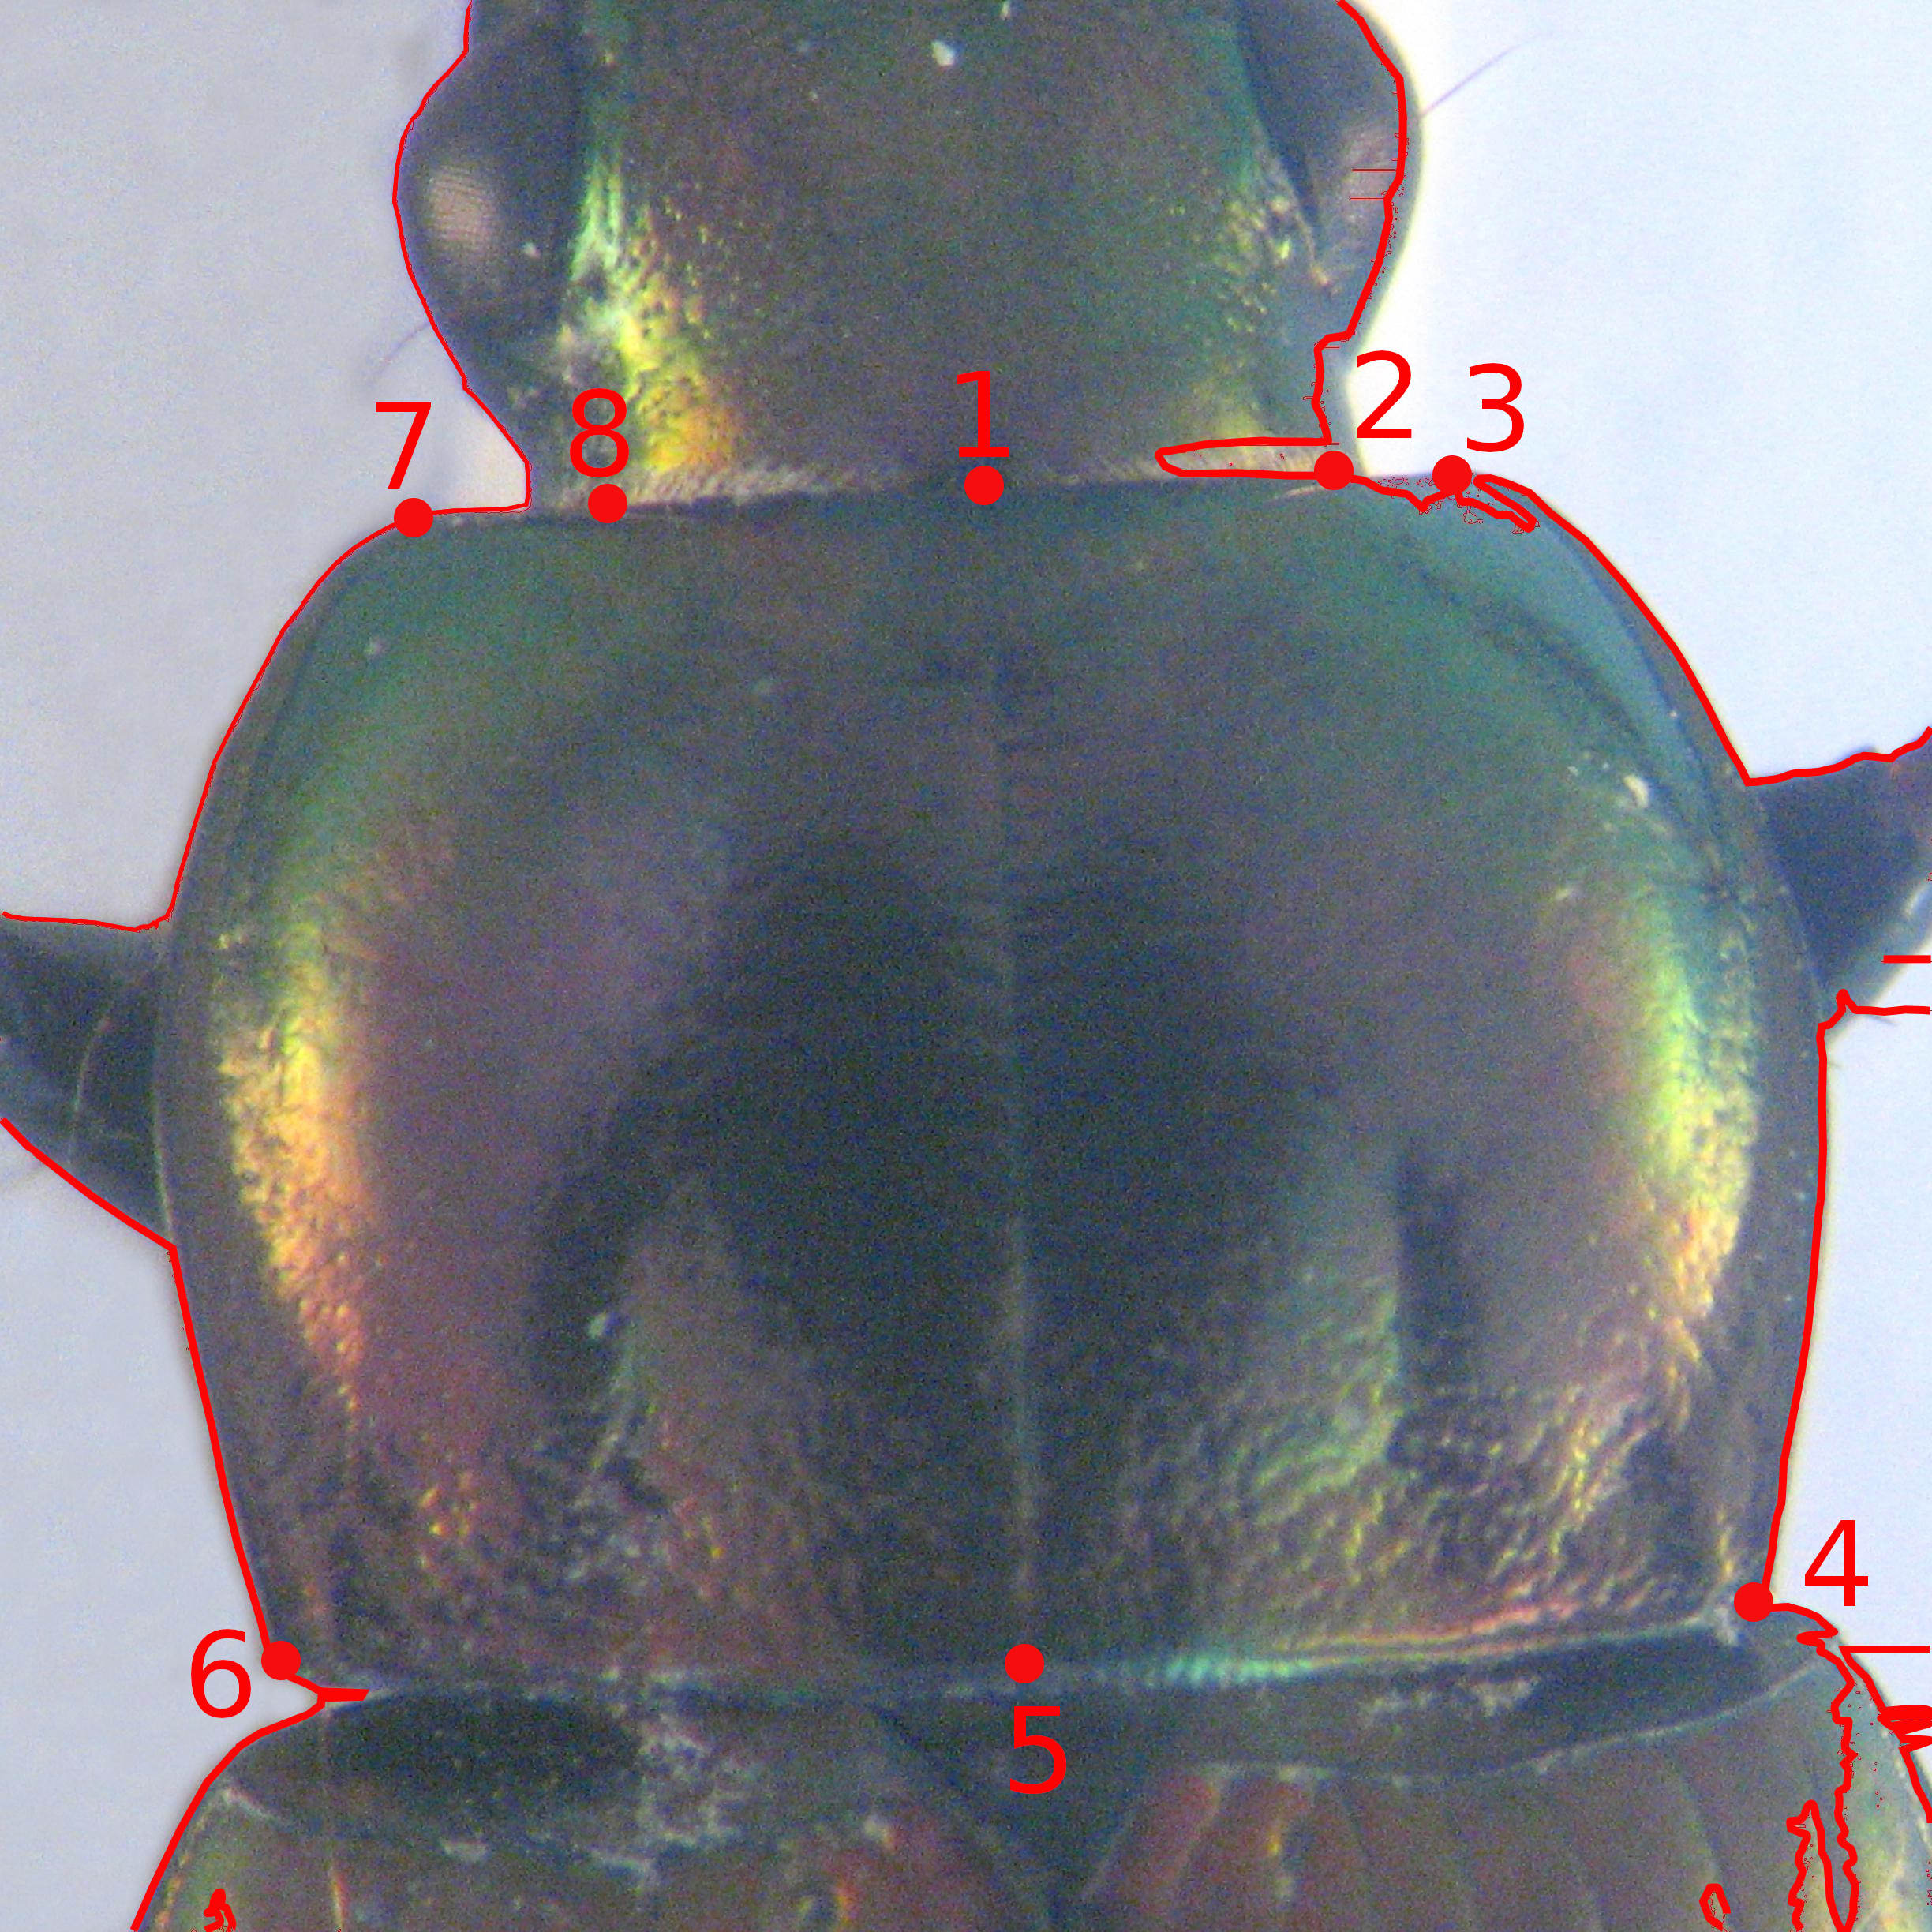
\includegraphics[scale=.055]{images/prono_003_lm2}
        }
        \only<2>{
        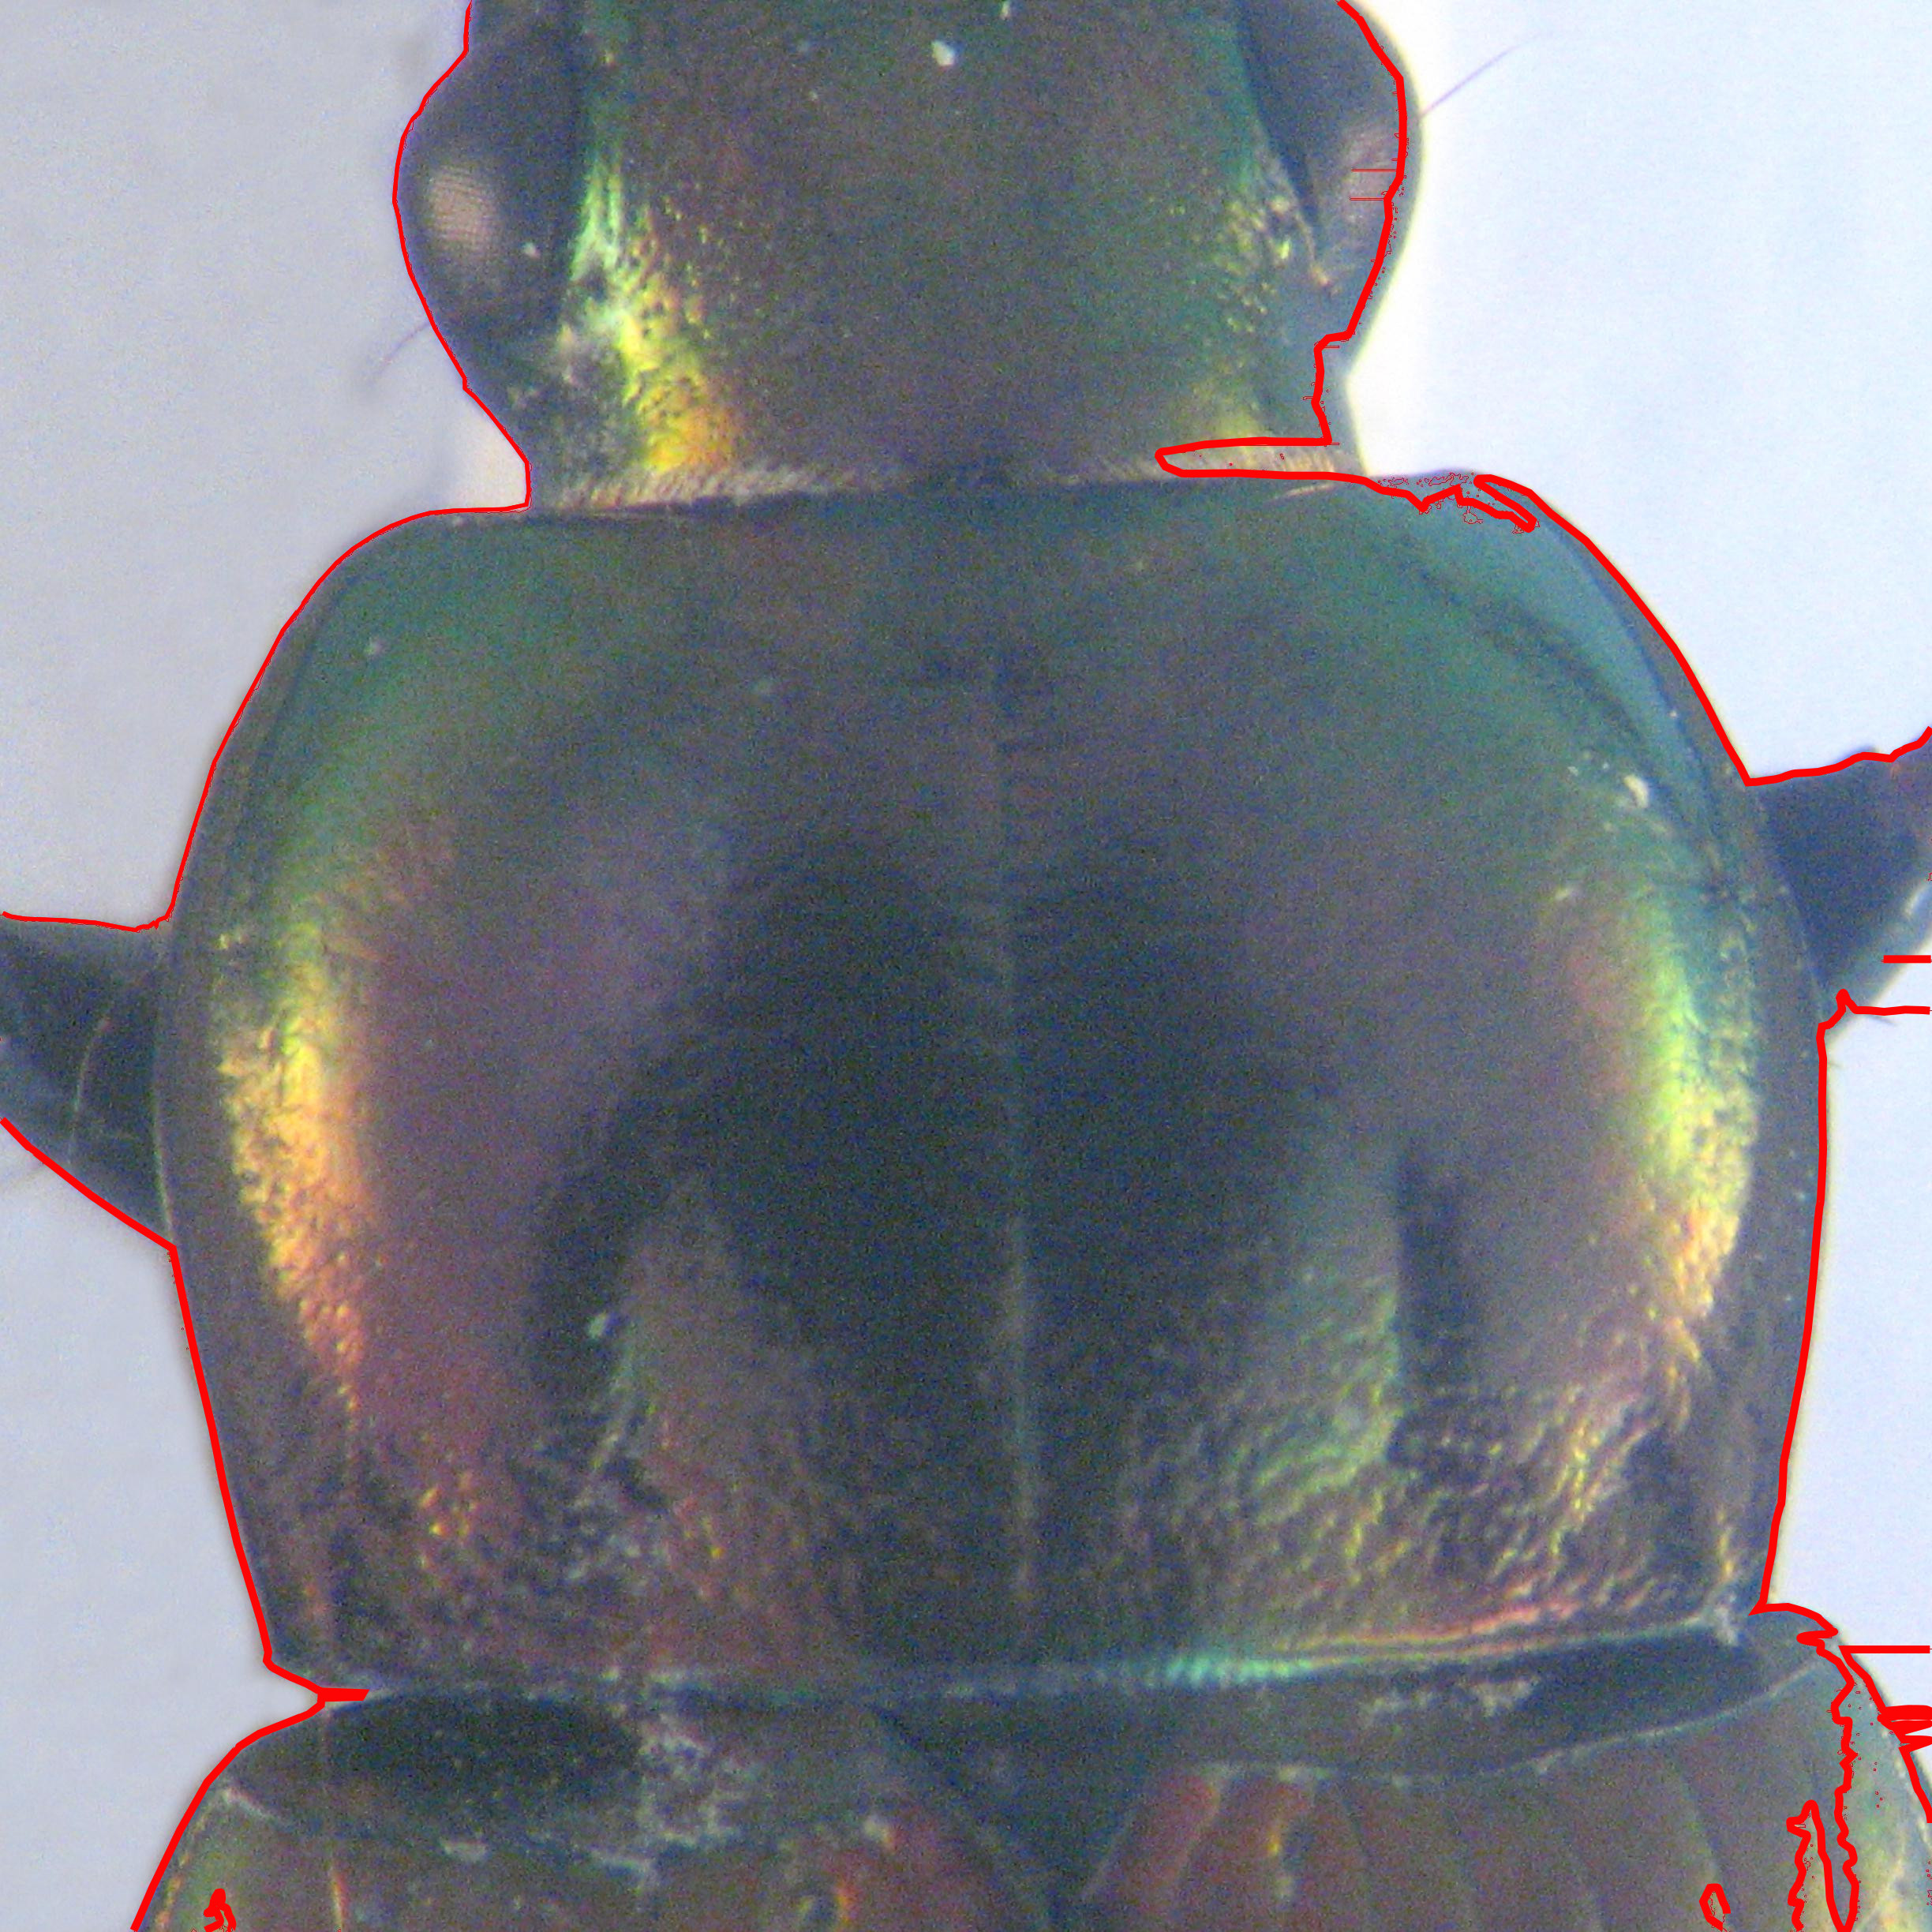
\includegraphics[scale=.055]{images/prono_003}
        }
        \only<2>{
        
\includegraphics[scale=.03]{images/arrow}
        }
        \only<2>
        {
        	\only<2>{\hspace{0cm}}
         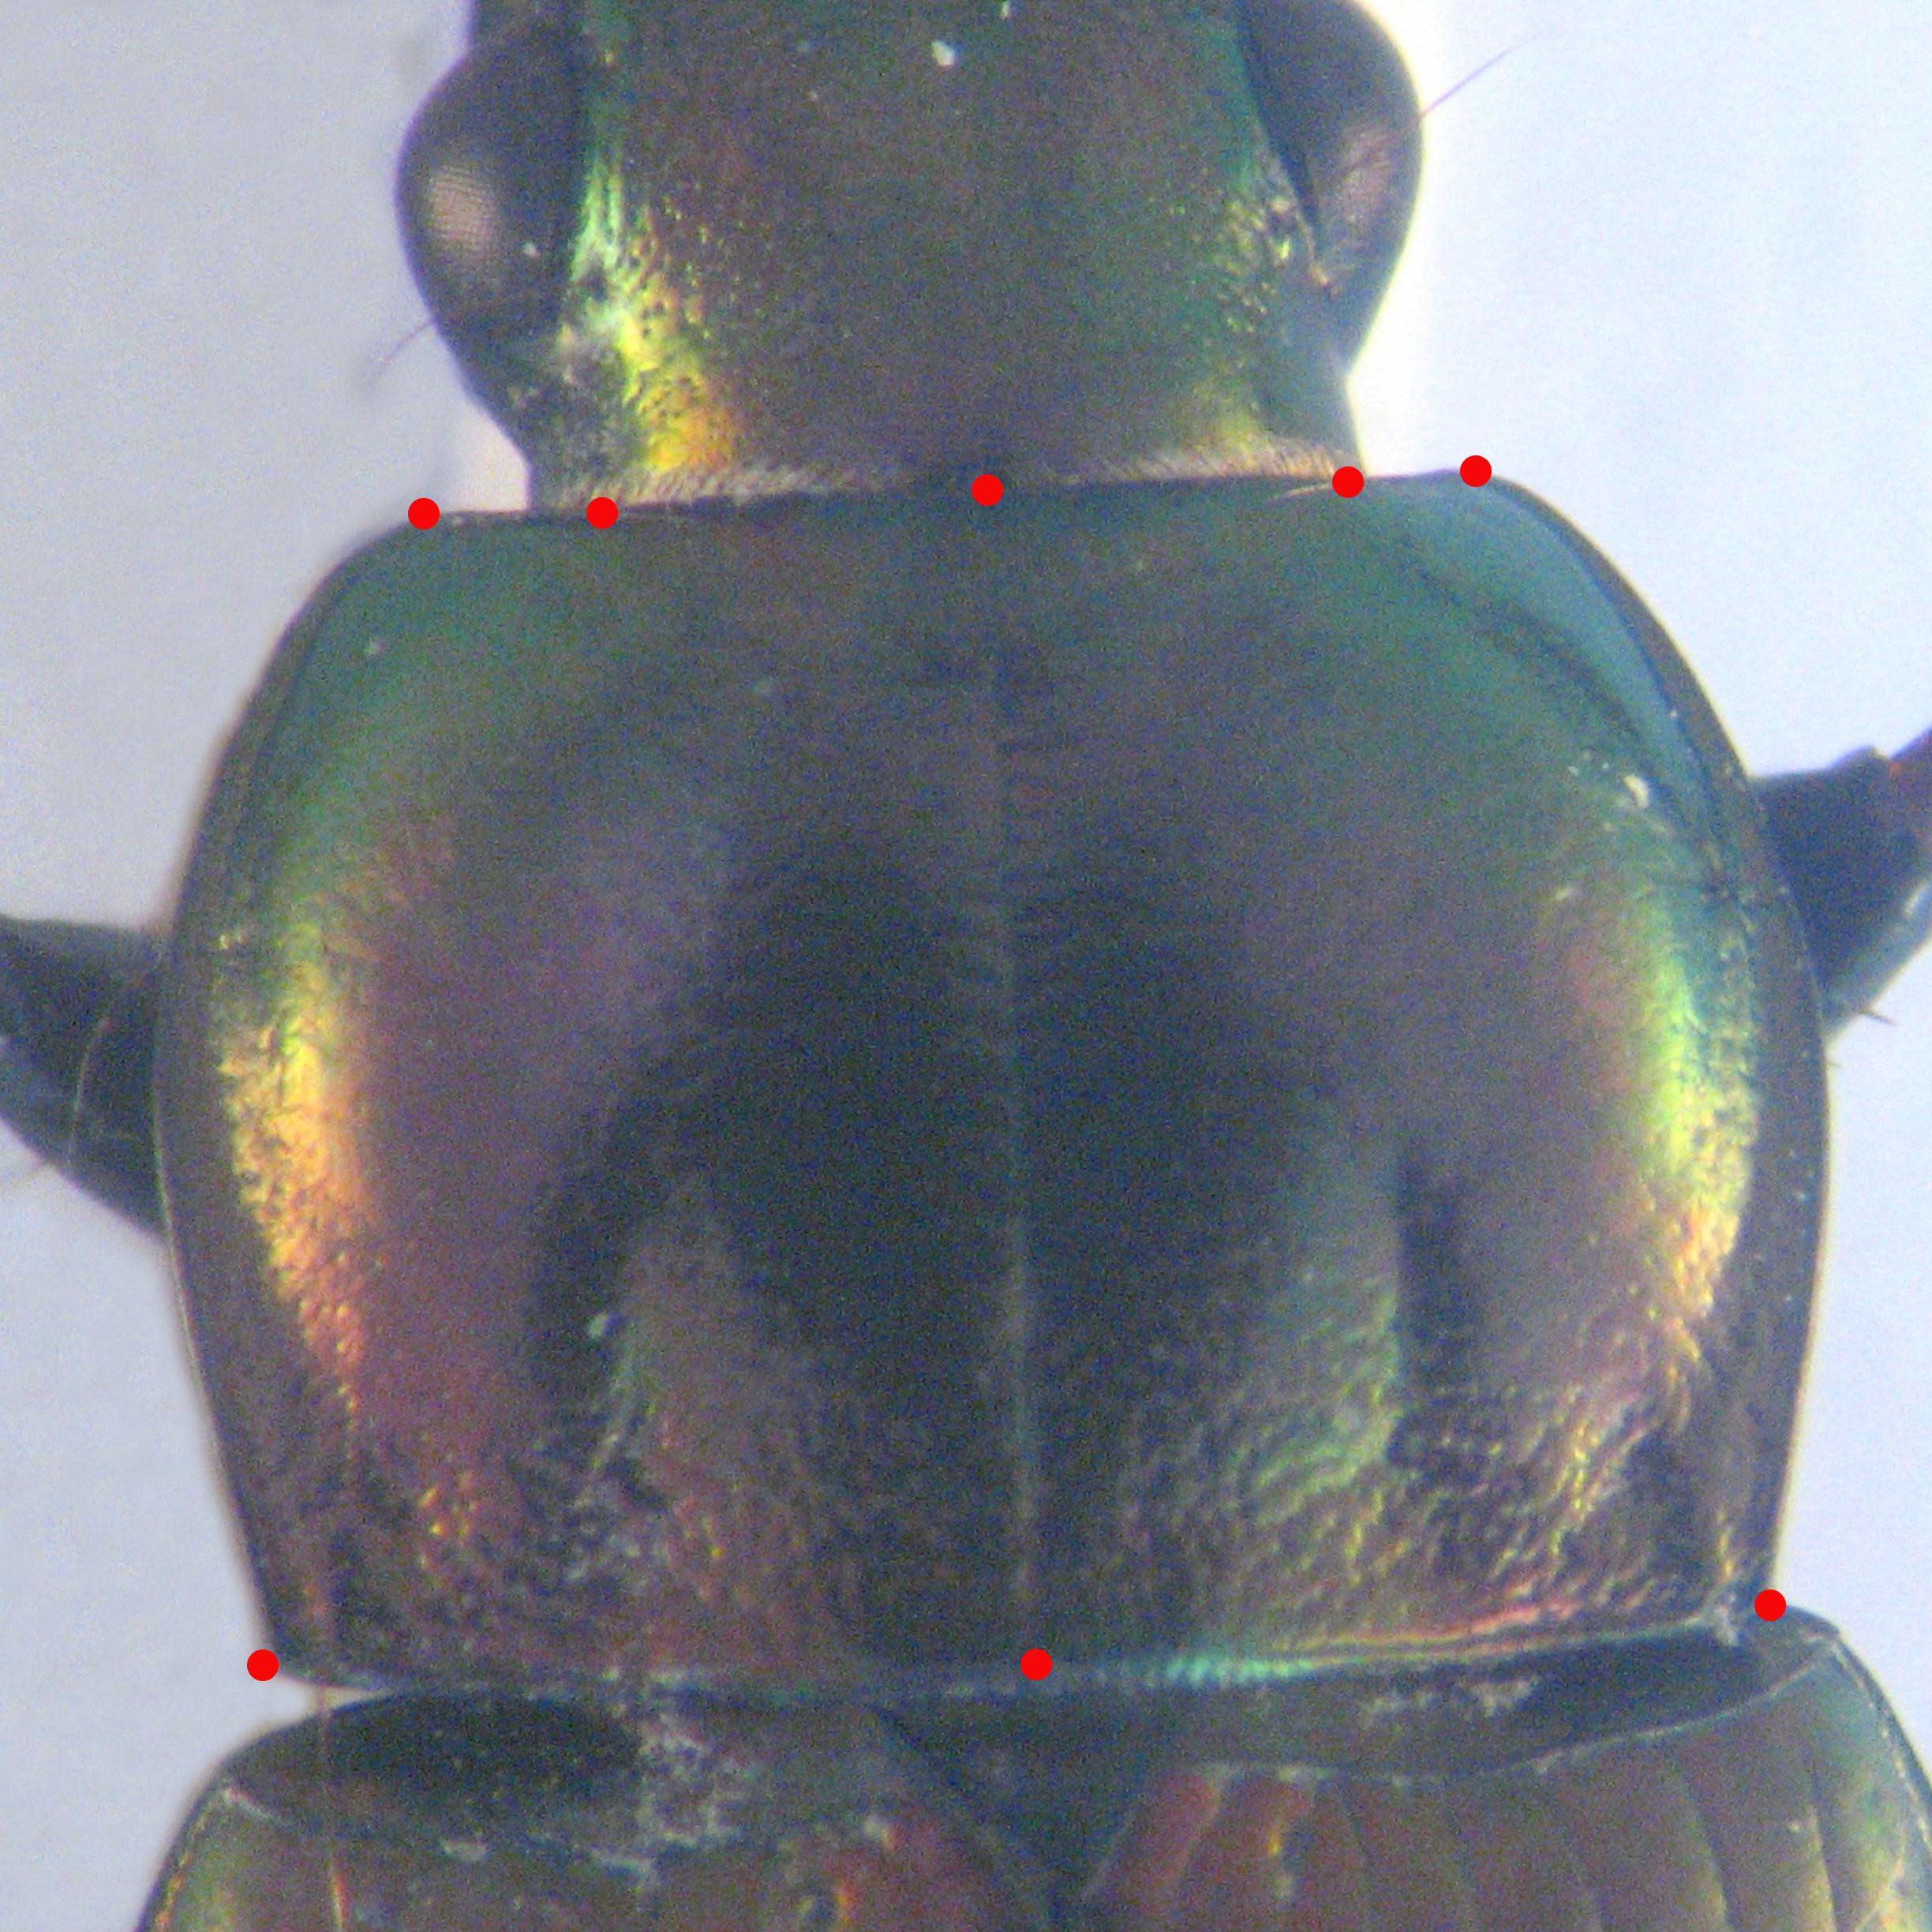
\includegraphics[scale=.055]{images/prono_003_lm}
         }
	\end{figure}
	\only<2>{
	\begin{center}	
		\textbf{How to {\color{red}automatically} predict the {\color{red}landmarks coordinates} on {\color{red}pronotum} images?}	
	\end{center}
	}
\end{frame}